\acresetall
\chapter{Live implementation in GNURadio}\label{chapter:live} \label{ch:live}

A live implementation of the scenario classification has been implemented using GNURadio. The models have been trained with the procedures explained in previous chapters and afterward its persistence is achieved using the sklearn library joblib for the feature-based learning and the library PyH5 for the spectrogram based learning.

The selection of the saved models is crucial for the good performance of the application. For the feature-based learning, the models with the best trade-off between validation accuracy and prediction time have been chosen. The selected models are:

\begin{itemize}
    \item K-nearest neighbors with 4 neighbors, trained with the whole (XL) unscaled dataset.
    \item A Decision tree with a tree depth=50, trained with the whole (XL) scaled dataset using a standard scaler.
    \item \ac{SVM} with an RBF complexity of \(\gamma=2^3\), trained with the medium (M) scaled dataset using a standard scaler.
\end{itemize}

For the spectrogram-based learning, an interesting technique is used for choosing the best fit for the real-time implementation. Keras provides routines for saving the model after the total of iterations is done, where one can assume that the model, after extensive training, will have an improving performance with increasing iteration number. However, a long training time can lead to overfitting of the model as seen at the end of section~\ref{ch:image_classification}. Two alternatives to avoid this are provided based on a constant callback of the accuracy and loss parameters. These alternatives are:

\begin{itemize}
    \item Early stopping: a monitored quantity can be selected from the accuracies or losses, and a range of improvement is set by the designer. Constantly, the selected value is checked, and everytime that it reaches a better performance a model's persistence is saved to disk. If there is no improvement in an arbitrary number of iterations thereafter, the process is stopped and the persistence of the model at the last iteration can also be saved to disk.
    \item Model Checkpoint: similarly to early stopping, a monitored quantity is selected, and the best model's persistence with respect to that quantity is saved to disk. However, the whole training process is run to completion, where the persistence of the model at the last iteration can also be saved to disk as well.
\end{itemize}

In this work model checkpoint was selected for model persistence, as it provides the capability of saving the best model with respect to a parameter as well as allowing the observation of the whole process by the cost of training times. The validation loss was selected as monitored quantity, as it represents how different was the predicted data to the training data, and considering that there is no significant improvement of accuracy after a couple hundreds of iterations for any of the models.

Simple blocks have been written to serve as a wrapper for the trained models, and a comparative setup with the implementation used at the DySpan Spectrum Challenge 2017 is carried out. As a first approach, the classification probabilities is extracted in real time. These probabilities state how certain is each of the algorithms at making a decision. For plotting, a modified "QT Time Raster" block is used, to see in the x-axis, ordinally, the possible scenarios from scenario 0 to 9, and the y-axis updates constantly to show outputs of the classifiers. It is important to notice that none of these axes reflect time directly, as it will become clear shortly. For testing, the \ac{PU} transmitter is set to send its packets using the scenarios increasingly for a duration of 2 seconds each. Additionally, different values of \ac{PU} transmission power have been used to determine the performance of the implemented machine learning algorithms facing different values of SNR. Fig~\ref{fig:prob_snr_15} shows these probability plots for an SNR=15dB.

\begin{figure}[!htb]
    \centering
      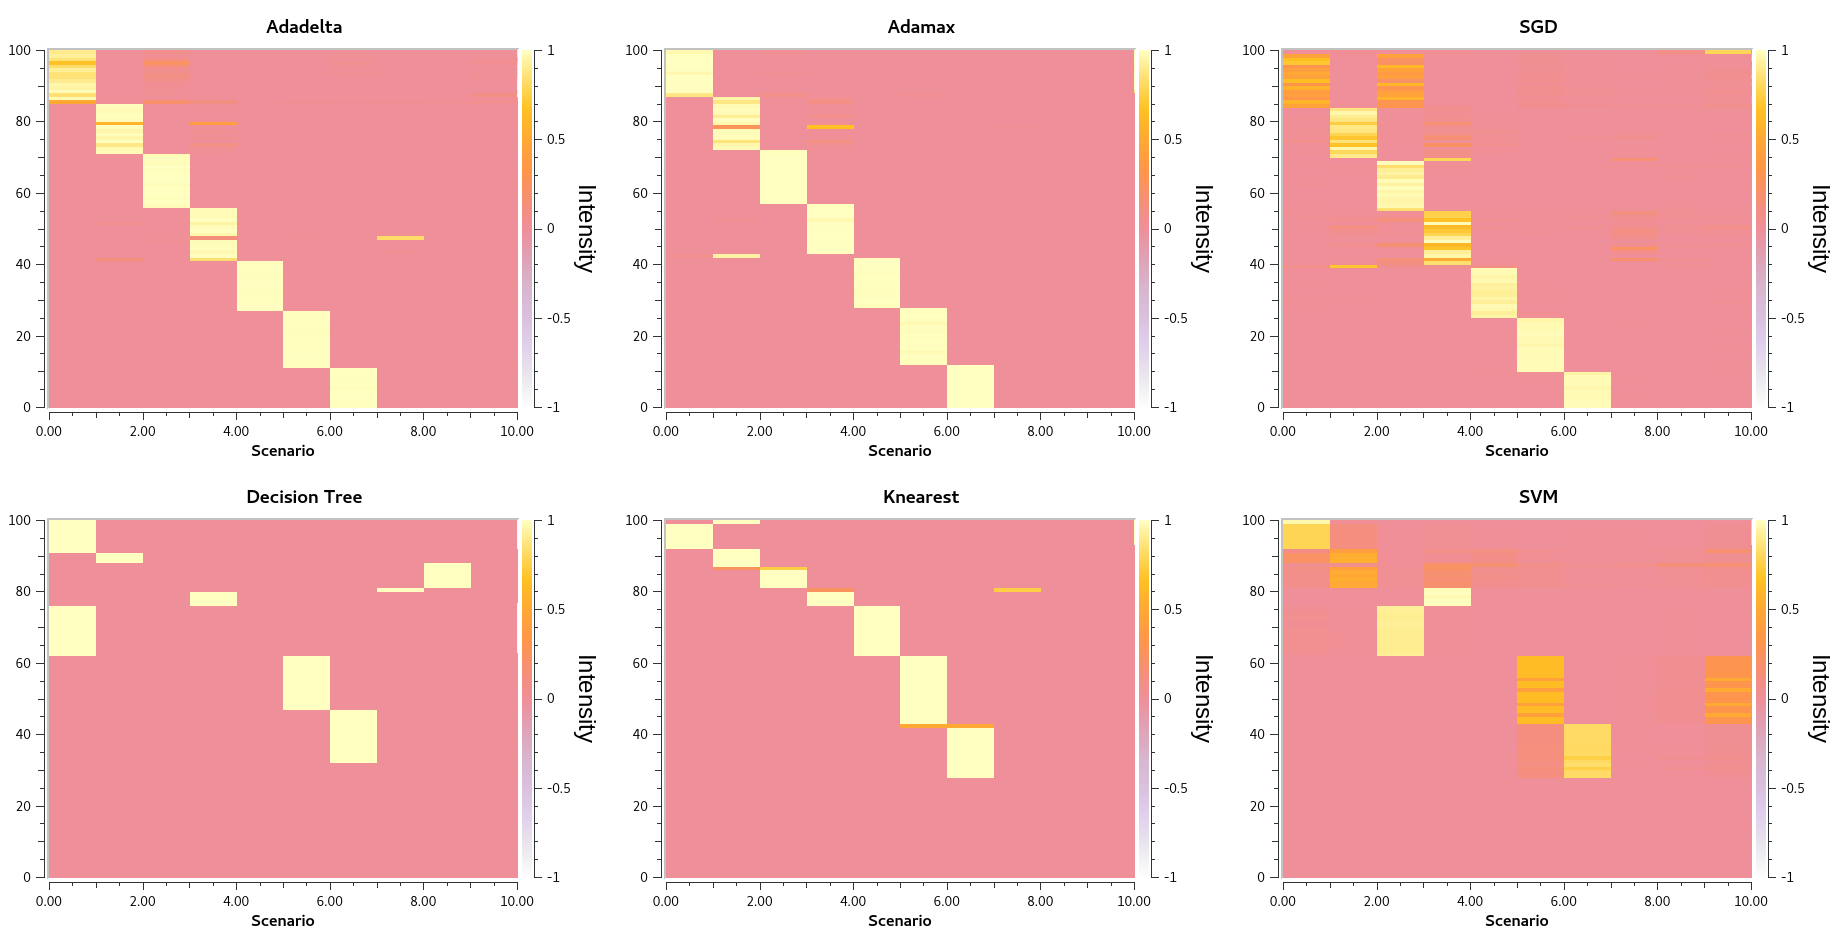
\includegraphics[width=\textwidth]{figures/prob_snr_15}
      \caption{Decision certainty for an SNR=15dB}
      \label{fig:prob_snr_15}
\end{figure}

The high intensity on these plots is represented with a lighter color and means a higher probability/certainty of a decision. In the top row the spectrogram-based algorithms are shown, and it can be seen that they show a consistent classification for each scenario every 2 seconds. Furthermore, the certainty of Adadelta and Adamax is clearer at the moment of making a decision vs. the certainty of SGD. However, this has little effect in the final result, as still the right scenario has a higher probability and is correctly classified, as seen in Fig~\ref{fig:scn_snr_15}. The row on the bottom shows the feature-based learning algorithms. On first instance it could be understood that they are not classifying correctly the scenarios, as a definite staircase-like fashion, as for the top row, is intuitively expected. However, it is important to notice that the nature of these classification models is different: it is feature based, while the top row is, so to say, sample based. What this means is that the top row classifies scenarios on the go based solely on the input data, whilst the bottom row classifies based on the frame events generated by the blocks described in Fig~\ref{fig:frame_events}. These frame events vary in quantity based on the number of frames that the \ac{PU} is transmitting, reason why in Fig~\ref{fig:scn_snr_15} the classified scenarios show to be longer for scenario 6 (high packet rate) than, for example, scenario 7 (low packet rate). This explains the difference on the output patterns.

\begin{figure}[!htb]
    \centering
      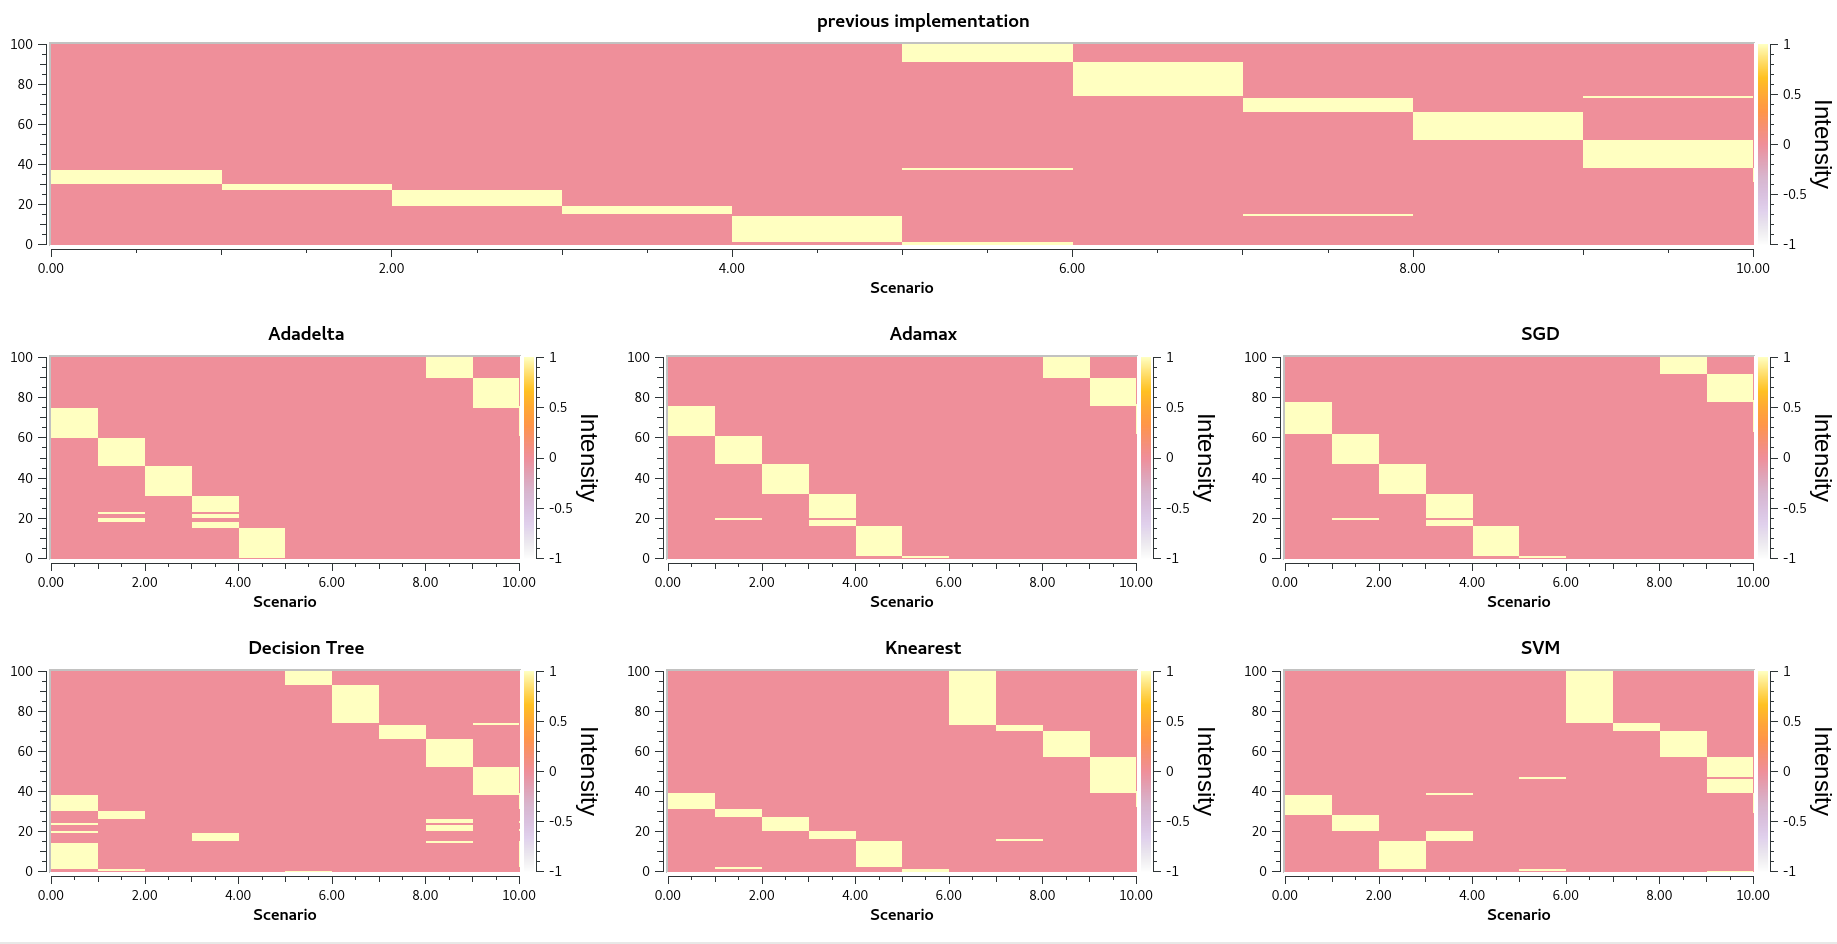
\includegraphics[width=\textwidth]{figures/scn_snr_15}
      \caption{Classified scenario for an SNR=15dB}
      \label{fig:scn_snr_15}
\end{figure}

In Fig~\ref{fig:scn_snr_15}, and in upcoming scenario classification figures, the implementation used in the DySpan Spectrum Challenge 2017 is plotted in the top row, moving the rows from Fig~\ref{fig:prob_snr_15} one position down. It can be seen that the pattern is alike to the feature-based classifiers, as they use the same features and frame events.

Additional plots for the decision probability and classified scenario are shown for SNR=10dB in Figs~\ref{fig:prob_snr_10}, \ref{fig:scn_snr_10}, SNR=5dB in Figs~\ref{fig:prob_snr_5}, ~\ref{fig:scn_snr_5} and SNR=0dB in Figs~\ref{fig:prob_snr_0}, \ref{fig:scn_snr_0}. An evident increase in the uncertainty can be seen with a decrease of the SNR, which is expected. Nevertheless, the spectrogram-based classifiers continue to have a remarkable performance even with low values of \ac{PU} transmit power. An important remark that cannot be seen in the pictures is that for SNR=5dB and below the frequency with which the frame events are generated decreases, given that they depend on detection of \ac{PU} energy. Because of this fact, all feature-based classifiers stop generating outputs consistently, until the point they just stop classifying (or generating outputs whatsoever). This sets a clear advantage for the spectrogram-based classifiers, as they are independent of the \ac{PU} transmission power.

\begin{figure}[!htb]
    \centering
      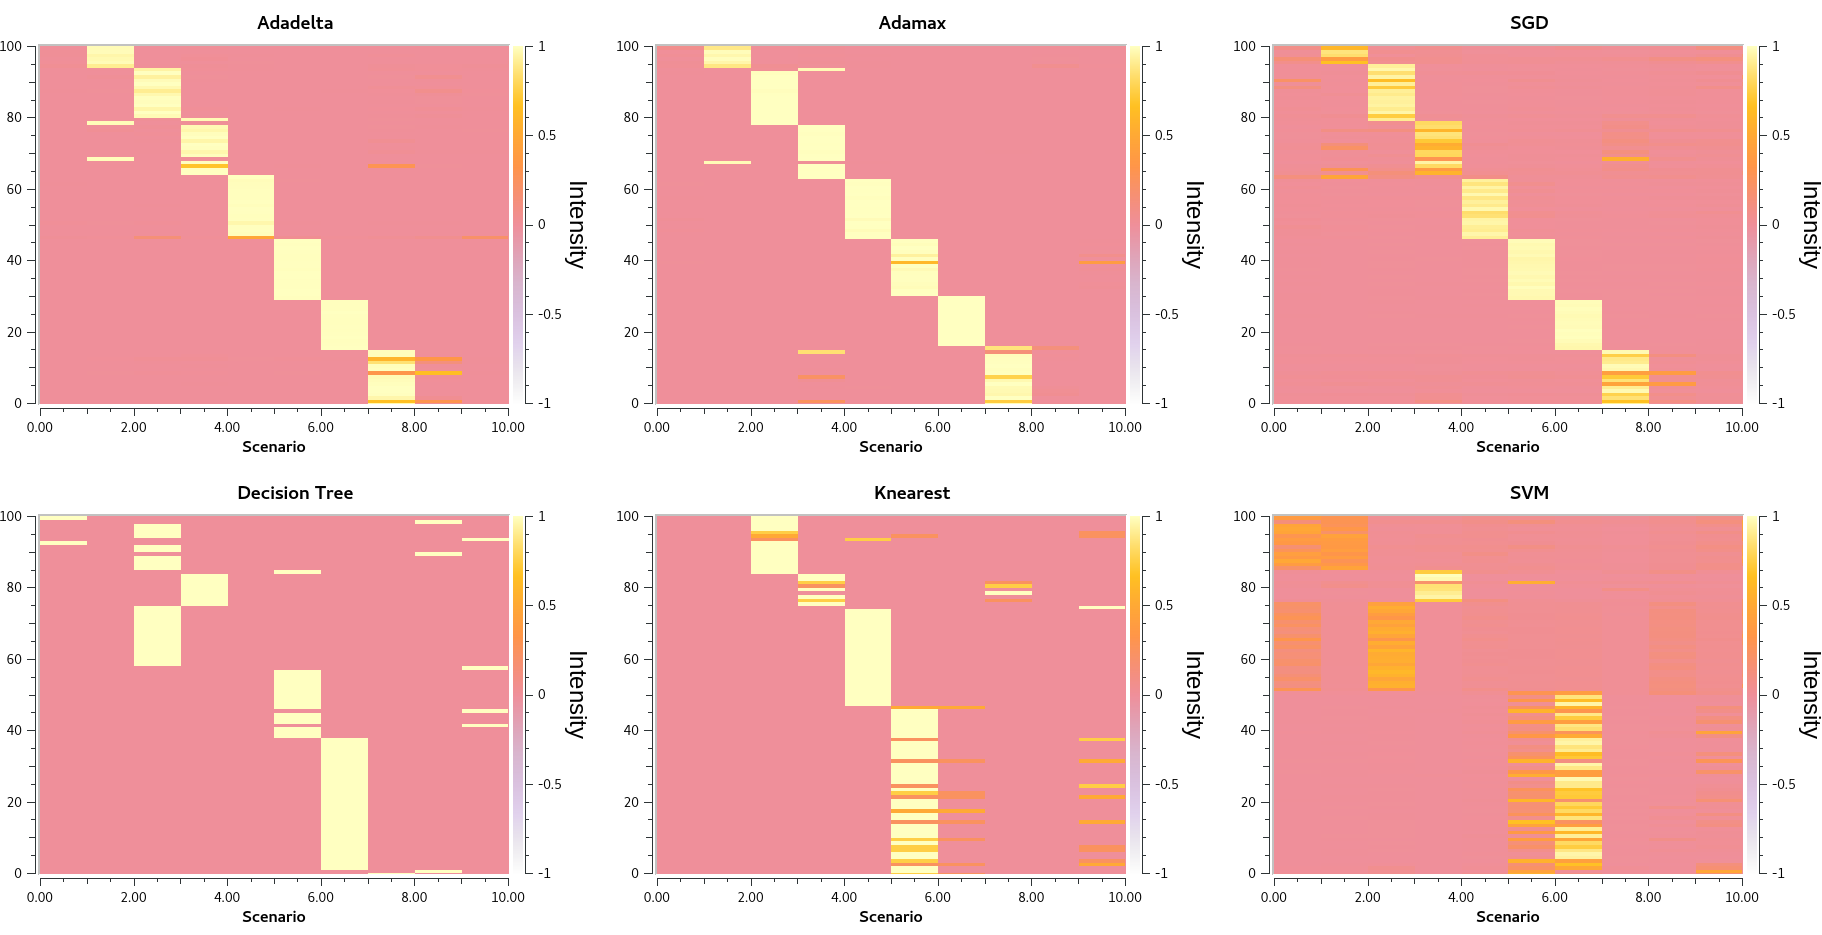
\includegraphics[width=\textwidth]{figures/prob_snr_10}
      \caption{Decision certainty for an SNR=10dB}
      \label{fig:prob_snr_10}
\end{figure}

\begin{figure}[!htb]
    \centering
      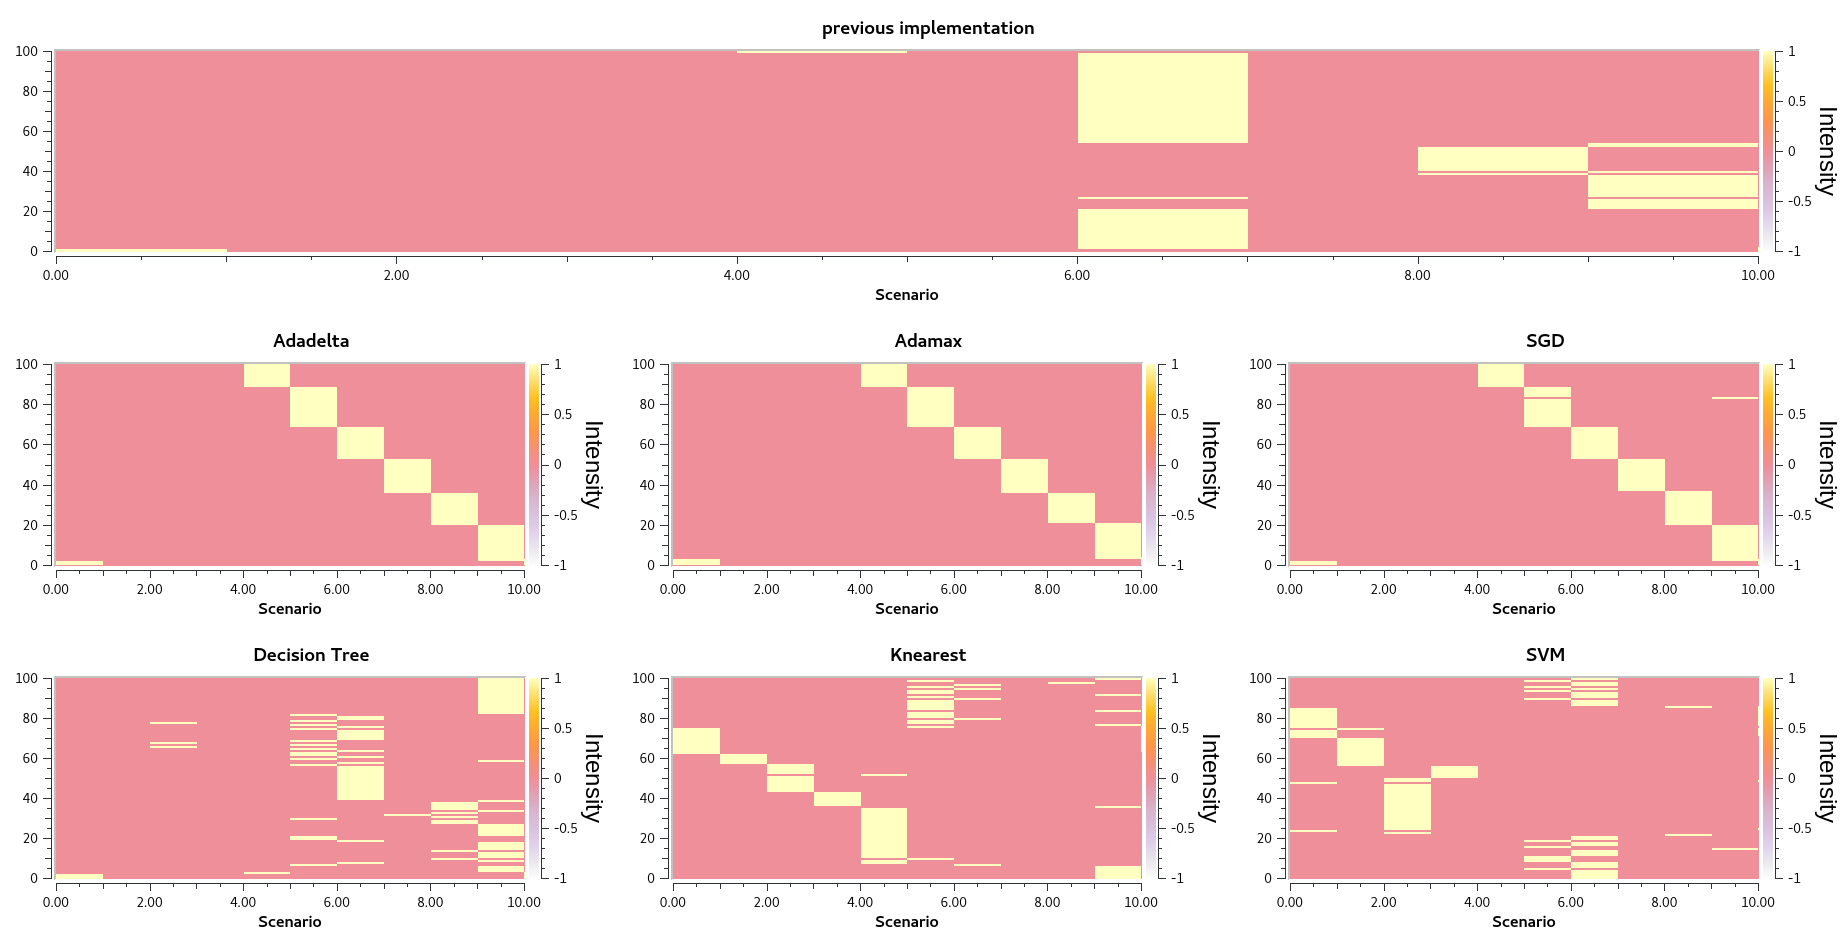
\includegraphics[width=\textwidth]{figures/scn_snr_10}
      \caption{Classified scenario for an SNR=10dB}
      \label{fig:scn_snr_10}
\end{figure}

\begin{figure}[!htb]
    \centering
      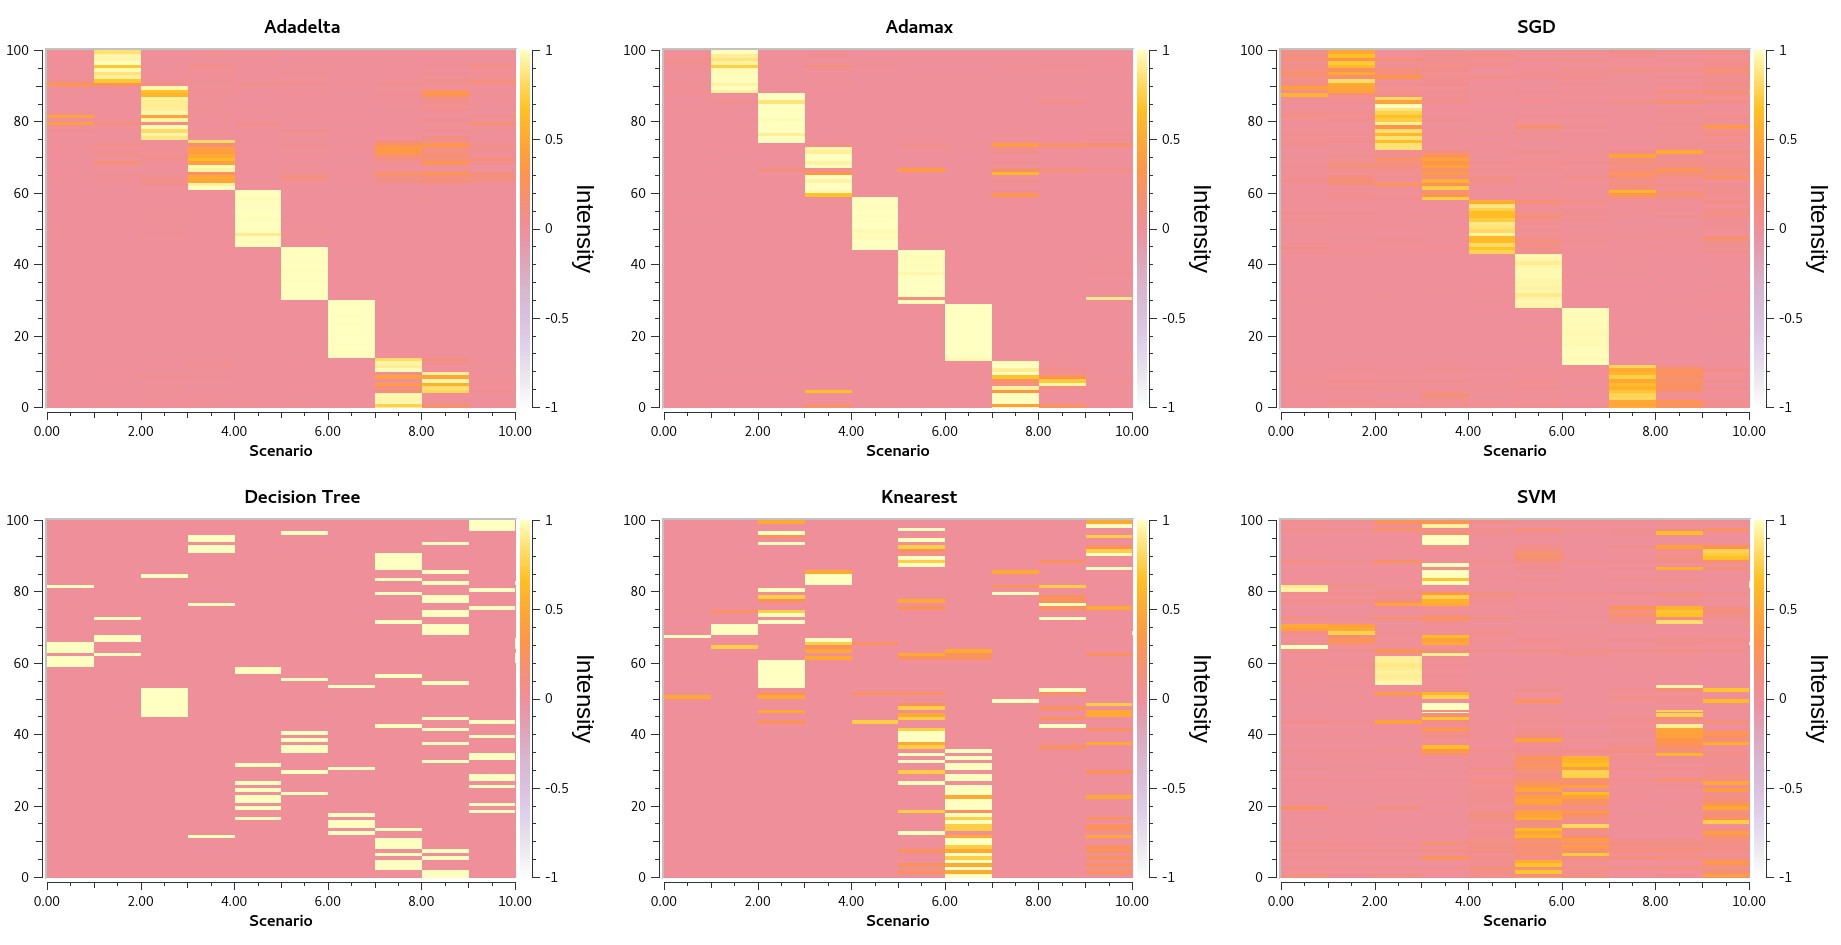
\includegraphics[width=\textwidth]{figures/prob_snr_5}
      \caption{Decision certainty for an SNR=5dB}
      \label{fig:prob_snr_5}
\end{figure}

\begin{figure}[!htb]
    \centering
      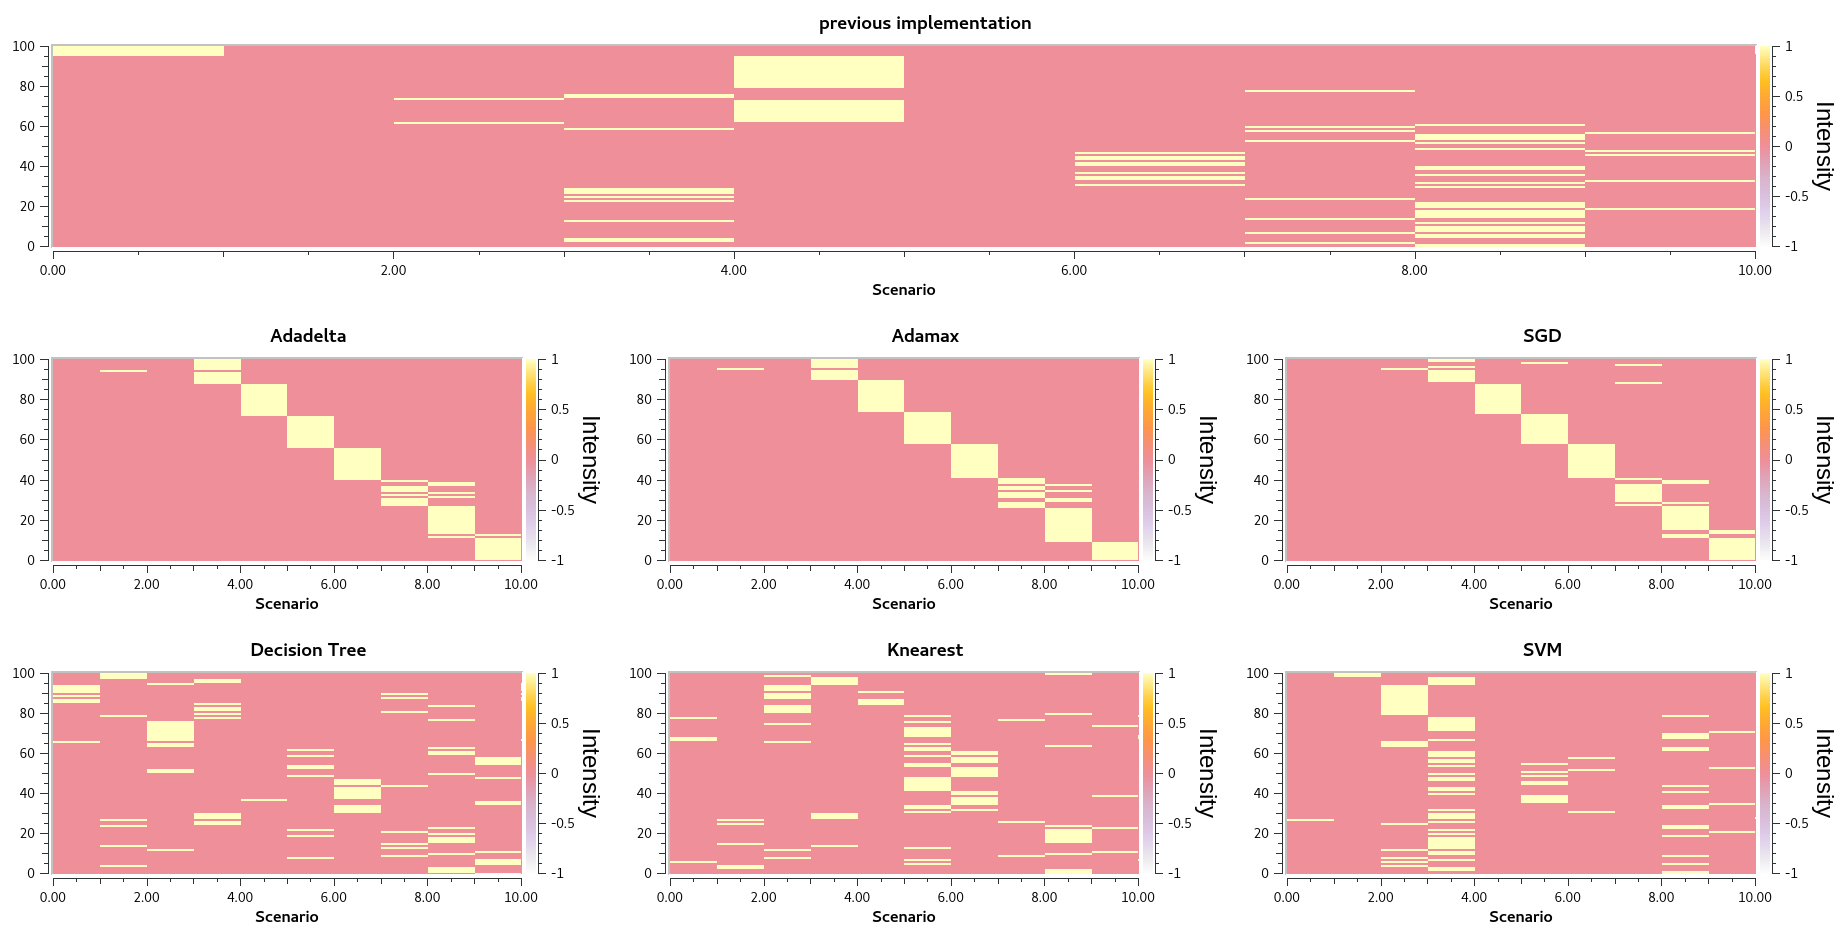
\includegraphics[width=\textwidth]{figures/scn_snr_5}
      \caption{Classified scenario for an SNR=5dB}
      \label{fig:scn_snr_5}
\end{figure}

\begin{figure}[!htb]
    \centering
      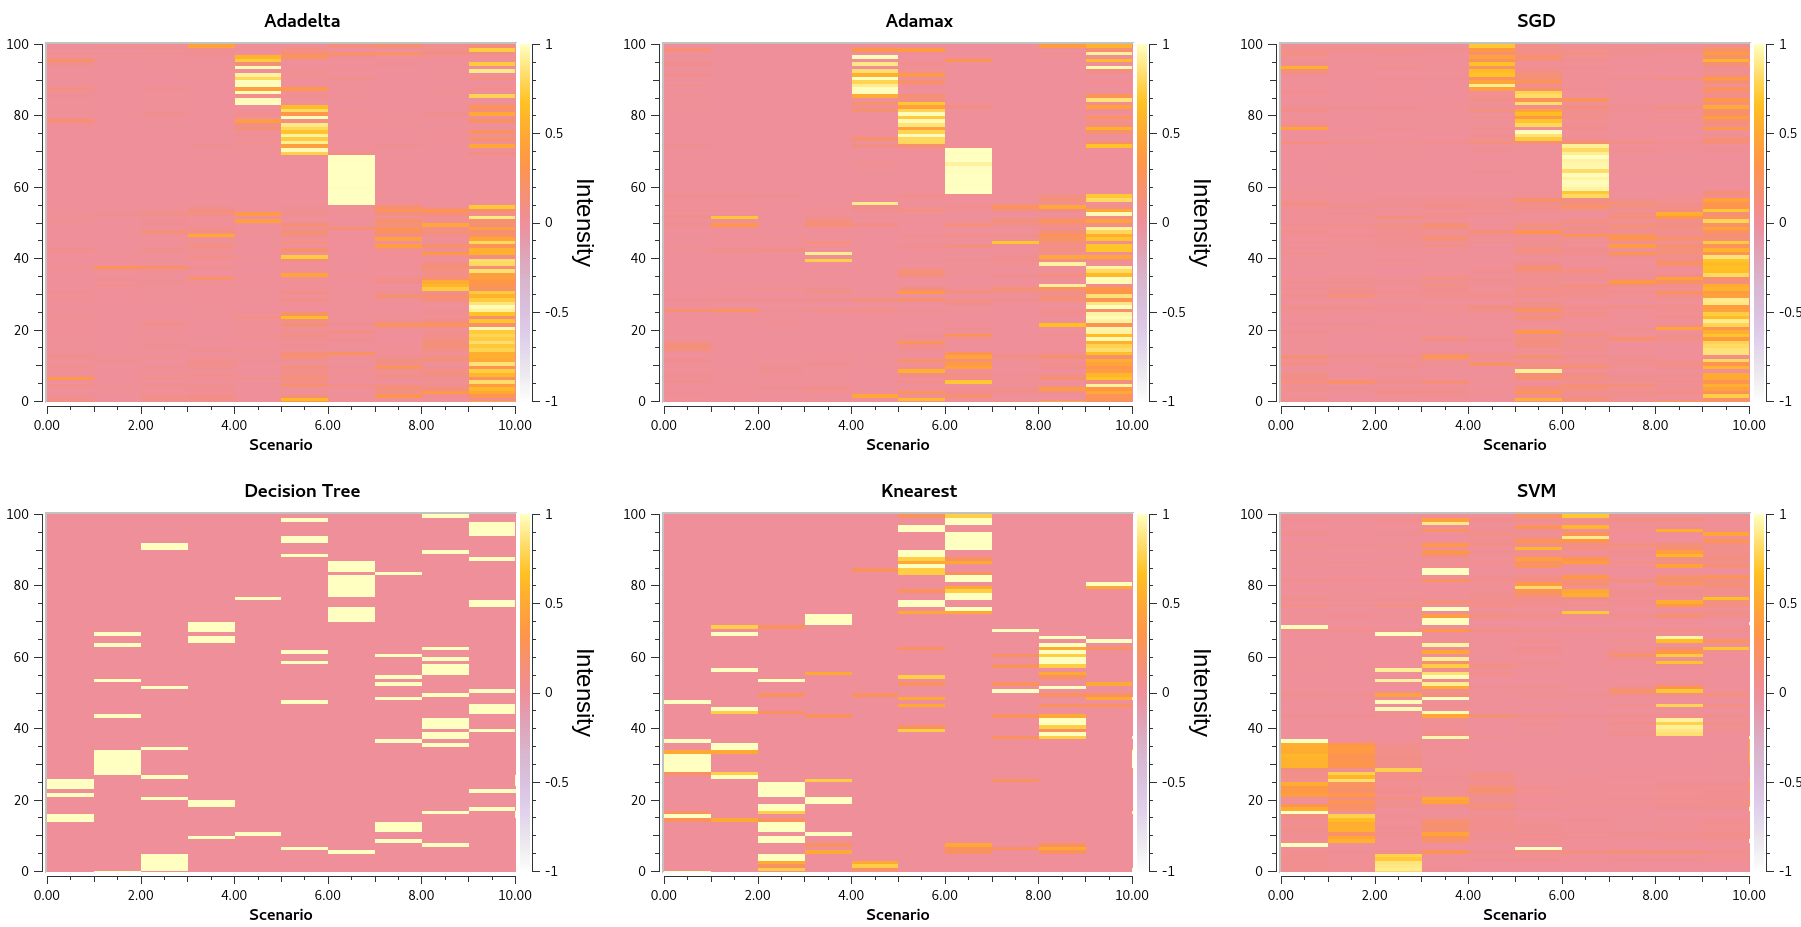
\includegraphics[width=\textwidth]{figures/prob_snr_0}
      \caption{Decision certainty for an SNR=0dB}
      \label{fig:prob_snr_0}
\end{figure}

\begin{figure}[!htb]
    \centering
      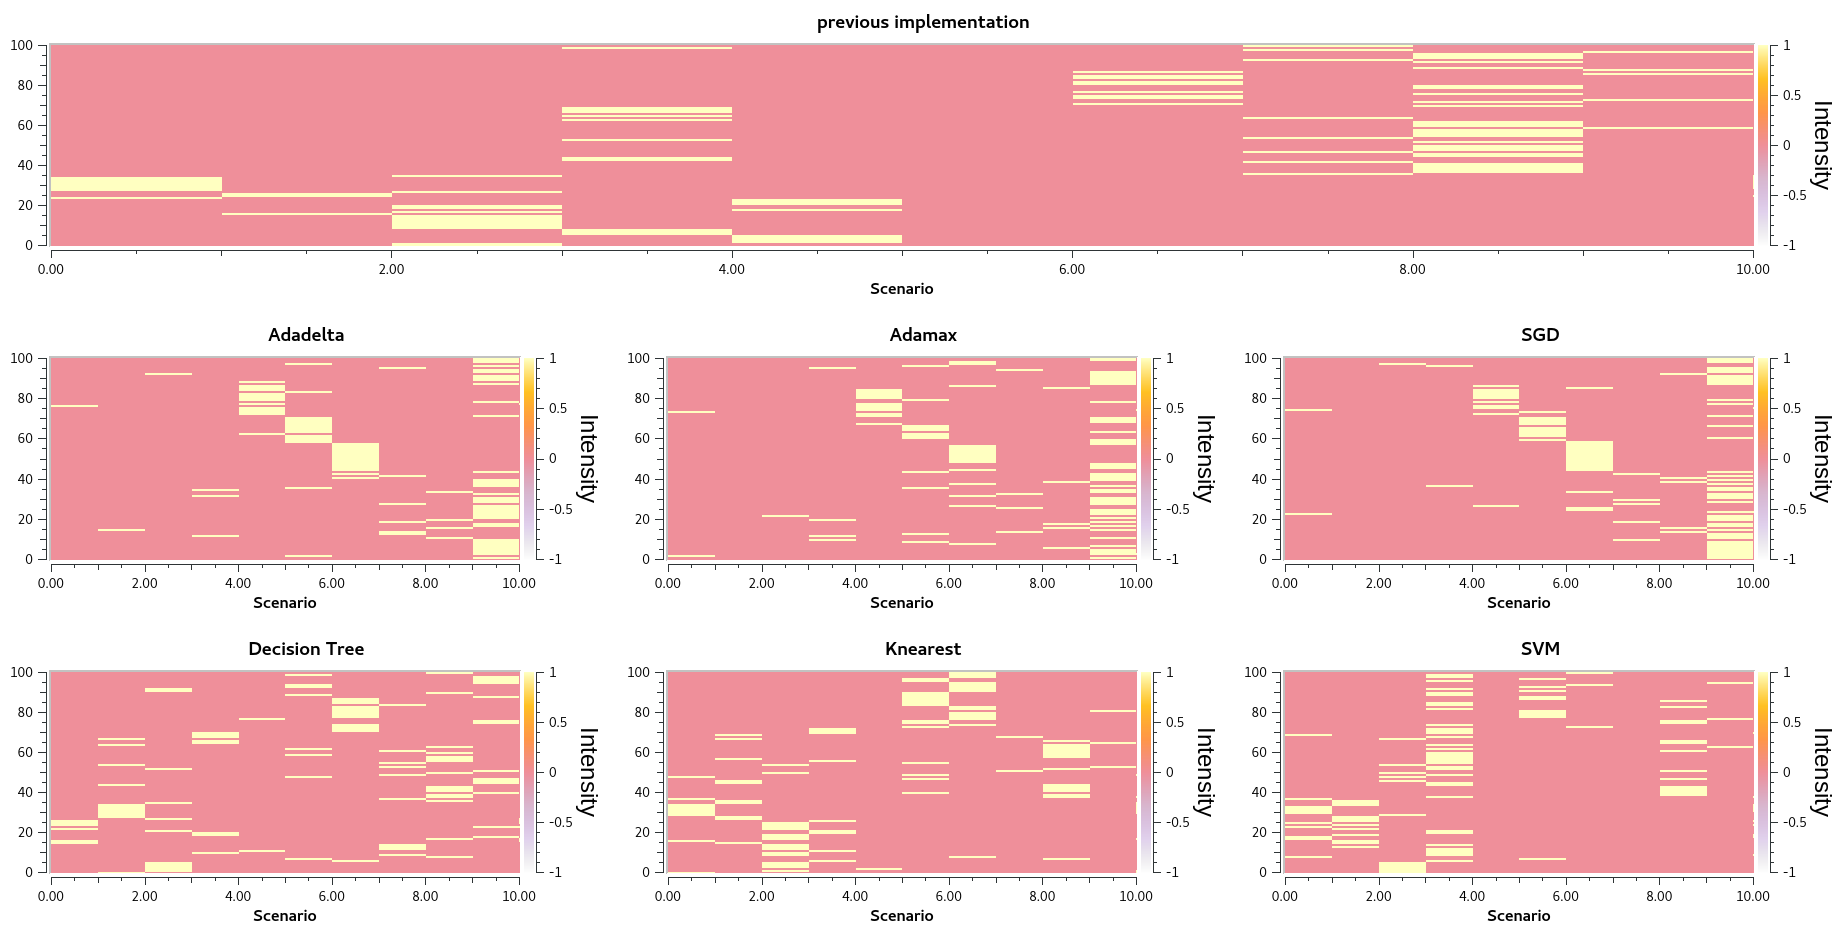
\includegraphics[width=\textwidth]{figures/scn_snr_0}
      \caption{Classified scenario for an SNR=0dB}
      \label{fig:scn_snr_0}
\end{figure}

